\chapter{Aplikácie}\label{chap:applications}

V tejto kapitole budeme prezentovať implementáciu vybraných štatistických modelov popísaných v predchádzajúcich kapitolách. Cieľom bolo nielen overiť ich teoretické vlastnosti, ale aj vytvoriť nástroje vhodné na praktickú prácu s dátami. Implementácia bola realizovaná v jazyku \texttt{R}, a to vo forme prehľadného a rozšíriteľného modulu, ktorý je sprístupnený prostredníctvom interaktívneho webového rozhrania (Shiny aplikácie).

\section{Regresný a klasifikačný model}\label{sec:app_regression_class}

V tejto časti prezentujeme implementáciu základných regresných a klasifikačných modelov, ktoré nám umožňujú odhadovať podmienenú strednú hodnotu a kvantilovú funkciu odozvy vzhľadom na zvolený prediktor. Cieľom týchto modelov je nielen získať rozdelenie odozvy, ale aj zachytiť nelineárne alebo neštandardné vzťahy v dátach.

\subsection{Implementácia regresných modelov}\label{subsec:regression_implementation}

Pre flexibilné modelovanie podmienenej závislosti medzi dvojicou premenných — spojitej odozvy $Y$ a prediktora $X$ (ktorý môže byť spojitý aj diskrétny) — bola implementovaná hlavná riadiaca funkcia \texttt{combine\_conditional\_models()}. Táto funkcia podľa typu vstupných premenných a používateľom zadaných parametrov zabezpečuje:

\begin{itemize}
  \setlength{\itemsep}{0pt}
  \setlength{\parskip}{0pt}
  \item výber vhodného regresného modelu pre odhad \textit{podmienenej strednej hodnoty} $\mathbb{E}[Y \mid X = x]$,
  \item odhad viacerých \textit{kvantilových funkcií} $Q_Y^{(X)}(q)$ pre zvolené úrovne kvantilu,
  \item spracovanie prípadov, kde je prediktor \textit{diskrétny} — výber medzi lineárnym a GLM prístupom,
  \item zjednotenú \textit{vizualizáciu} (regresné krivky, odhady v konkrétnom bode $x^*$),
  \item a sumarizáciu výstupov v prehľadných tabuľkách typu \texttt{gt}.
\end{itemize}

Funkcia tiež obsahuje vstavanú validáciu vstupov, automaticky rozpoznáva typ premenných a v prípade potreby ich transformuje na číselné. Výpočtové časti deleguje na nižšie opísané pomocné moduly podľa zvolených metód modelovania.

\subsubsection{Modelovanie podmienenej strednej hodnoty}\label{subsec:app_cond_mean}

Odhad podmienenej strednej hodnoty $\mathbb{E}[Y \mid X = x]$ je zabezpečený pomocou funkcie \texttt{model\_conditional\_mean()}, ktorá podporuje nasledovné metódy:

\begin{itemize}
  \item \textbf{Parametrické modely:}
  \begin{itemize}
  \setlength{\itemsep}{0pt}
  \setlength{\parskip}{0pt}
    \item "\texttt{linear}" – klasická lineárna regresia,
    \item "\texttt{poly}" – polynomiálna regresia (vyžaduje stupeň \texttt{poly\_mean\_degree}),
    \item "\texttt{exp}" – exponenciálny model $Y = a \cdot \exp(bX)$ (fitovaný cez \texttt{nls}),
    \item "\texttt{spline}" – B-spline bázy s počtom stupňov voľnosti \texttt{df = 5}.
  \end{itemize}
  \item \textbf{Neparametrické modely:}
  \begin{itemize}
  \setlength{\itemsep}{0pt}
  \setlength{\parskip}{0pt}
    \item "\texttt{loess}" – lokálne vyhladzovaný model (LOESS, \texttt{span = 0.75}),
    \item "\texttt{gam}" – generalizovaný aditívny model s hladkou spline funkciou (\texttt{mgcv::gam}).
  \end{itemize}
\end{itemize}

Funkcia vracia predikovanú hodnotu podmienenej strednej hodnoty pre celú mriežku hodnôt prediktora, ako aj konkrétnu hodnotu $\mathbb{E}[Y \mid X = x^*]$ pre zvolenú hodnotu $x^*$. Súčasťou výstupu je aj tabuľka s metrikami kvality modelu (R$^2$, MSE) a prípadne aj s parametrami modelu (odhad ± štandardná chyba).

\subsubsection{Modelovanie podmienenej kvantilovej funkcie}\label{subsec:app_cond_quantile}

Podmienené kvantilové funkcie $Q_Y^{(X)}(q)$ sú odhadované pomocou funkcie \texttt{model\_conditional\_quantiles()}, ktorá umožňuje odhad pre viaceré kvantily naraz. Podporované metódy sú:

\begin{itemize}
\setlength{\itemsep}{0pt}
  \setlength{\parskip}{0pt}
  \item \texttt{"linear"} – lineárna kvantilová regresia,
  \item \texttt{"poly"} – kvantilová regresia s polynomiálnou bázou (vyžaduje \texttt{poly\_quant\_degree}),
  \item \texttt{"spline"} – kvantilová regresia s B-spline funkciou (\texttt{df = 4}).
\end{itemize}

Výstupom je dátová tabuľka so všetkými vypočítanými hodnotami $Q_q(Y \mid X = x)$ pre každý kvantil $q$ a mriežku hodnôt $x$, ako aj samostatné bodové odhady pre konkrétne $x^*$. Súčasťou výstupu sú tiež tabuľky so štatistikami a parametrami každého modelu: odhady, chyby, AIC, deviance atď.

\subsubsection{Modelovanie pri diskrétnom prediktore}\label{subsec:app_discrete_pred}

V prípade, že prediktor $X$ je diskrétneho typu (napr. faktor alebo textová premenná), funkcia \texttt{combine\_conditional\_models()} automaticky použije modul \texttt{model\_discrete\_predictor()}, ktorý podporuje:

\begin{itemize}
\setlength{\itemsep}{0pt}
  \setlength{\parskip}{0pt}
  \item \texttt{"lm"} – klasický lineárny model so zaobchádzaním s faktormi,
  \item \texttt{"glm\_log"} – GLM model s logaritmickou linkou pre pozitívne odozvy.
\end{itemize}

Vizualizácia je realizovaná pomocou boxplotu s naznačenými bodovými odhadmi $\mathbb{E}[Y \mid X = d_k]$ a príslušnými intervalmi spoľahlivosti. Súčasťou výstupu sú aj štandardné regresné tabuľky s parametrami a R$^2$.

\subsubsection{Zhrnutie funkcionality}

Všetky moduly regresného modelovania sú implementované ako samostatné funkcie s jednotným rozhraním, čo umožňuje ich nezávislé testovanie a využitie. Riadiaca funkcia \texttt{combine\_conditional\_models()} zabezpečuje výber správneho postupu podľa typu vstupných premenných a parametrov. Vizualizácie sú vytvárané pomocou balíka \texttt{ggplot2} a sumarizačné výstupy vo forme prehľadných tabuliek pomocou \texttt{gt}.

Významnou vlastnosťou je aj jednotné spracovanie bodových odhadov pre konkrétnu hodnotu prediktora $x^*$, ktoré sú automaticky počítané pre oba typy modelov (stredná hodnota aj kvantily) a vizuálne vyznačené na grafe.


\subsection{Implementácia klasifikačných modelov}\label{subsec:classification_implementation}

Na modelovanie diskrétnej (kategoriálnej) odozvy vzhľadom na jeden alebo dva prediktory bola implementovaná univerzálna funkcia \texttt{classification\_model()}, ktorá pokrýva najpoužívanejšie klasifikačné prístupy. Používateľ si môže zvoliť vhodnú metódu podľa typu údajov a požiadaviek na interpretáciu alebo flexibilitu modelu.

Táto funkcia umožňuje používateľovi jednoducho:

\begin{itemize}
\setlength{\itemsep}{0pt}
  \setlength{\parskip}{0pt}
  \item špecifikovať typ klasifikačnej metódy (logistická regresia, LDA, QDA, KNN),
  \item modelovať úlohy s jedným prediktorom (dodatočne aj s dvomi),
  \item automaticky zvoliť optimálny počet susedov pre KNN (ak nie je zadaný),
  \item vizualizovať rozhodovacie hranice alebo klasifikačné prahy,
  \item získať sumarizáciu výkonu modelu a odhadnutých parametrov.
\end{itemize}

\subsubsection{Podporované metódy klasifikácie}

Funkcia \texttt{classification\_model()} podporuje nasledovné typy modelov:

\begin{itemize}
\setlength{\itemsep}{0pt}
  \setlength{\parskip}{0pt}
  \item \textit{Logistická regresia} ("\texttt{logistic}") – vhodná pre binárne aj multinomické klasifikačné úlohy. Binarizácia prebieha automaticky podľa počtu úrovní cieľovej premennej.
  \item \textit{Lineárna diskriminačná analýza ("\texttt{lda}")} – predpokladá rovnaké kovariančné matice naprieč triedami.
  \item \textit{Kvadratická diskriminačná analýza ("\texttt{qda}")} – umožňuje odlišné kovariančné štruktúry pre jednotlivé triedy. Triedy s menej ako štyrmi pozorovaniami sú automaticky vyradené.
  \item \textit{K najbližších susedov ("\texttt{knn}")} – výber optimálneho $k$ v rozsahu $1 \leq k \leq 20$ na základe maximalizácie presnosti.
\end{itemize}

\subsubsection{Vstupné a výstupné prvky}

Funkcia vyžaduje nasledovné vstupné argumenty:

\begin{itemize}
\setlength{\itemsep}{0pt}
  \setlength{\parskip}{0pt}
  \item \texttt{data} – dátový rámec so vstupnými premennými,
  \item \texttt{response\_name} – meno cieľovej premennej (diskrétna),
  \item \texttt{predictor\_names} – meno jedného prediktora (umožňuje však aj dva),
  \item \texttt{method} – typ modelu (napr. \texttt{"logistic"}, \texttt{"qda"}, ...),
  \item \texttt{k} – počet susedov pre KNN (voliteľné).
\end{itemize}

Výstupom funkcie je štruktúrovaný zoznam s nasledujúcimi komponentmi:

\begin{itemize}
\setlength{\itemsep}{0pt}
  \setlength{\parskip}{0pt}
  \item \texttt{model} – fitovaný klasifikačný model,
  \item \texttt{predictions} – vektor predikovaných tried,
  \item \texttt{accuracy} – presnosť modelu na trénovacej množine,
  \item \texttt{confusion\_matrix} – matica zámien (confusion matrix),
  \item \texttt{summary\_gt} – sumarizačná tabuľka v štýle \texttt{gt} s parametrami modelu,
  \item \texttt{decision\_plot} – vizualizácia rozhodovacích hraníc (ak počet prediktorov $\leq 2$).
\end{itemize}

\subsubsection{Vizualizácia}

Výsledky klasifikácie sú doplnené aj o interaktívnu vizualizáciu:

\begin{itemize}
\setlength{\itemsep}{0pt}
  \setlength{\parskip}{0pt}
  \item Pri jednom prediktore sa zobrazuje rozhodovací prah a podmienené pravdepodobnosti (pomocou funkcie \texttt{plot\_classification\_1D\_combined()}).
  \item Pri dvoch prediktoroch sa vykreslí rozhodovacia hranica v prediktorovom priestore (pomocou funkcie \texttt{plot\_decision\_boundary()}).
\end{itemize}

\subsubsection{Sumarizačná tabuľka}

Súčasťou každého modelu je prehľadná sumarizačná tabuľka obsahujúca:

\begin{itemize}
\setlength{\itemsep}{0pt}
  \setlength{\parskip}{0pt}
  \item názov použitej metódy,
  \item celkovú presnosť klasifikácie,
  \item (ak sú dostupné) parametre $\beta$ so štandardnými chybami,
  \item pre LDA/QDA: priemery a smerodajné odchýlky podľa tried.
\end{itemize}

Táto implementácia ponúka užívateľsky jednoduchý, ale výpočtovo robustný nástroj na vizuálne aj kvantitatívne porovnanie rôznych klasifikačných metód v závislosti od typu dát.


\section{Odhad združeného rozdelenia}\label{sec:joint_dist_estimation}

V tejto kapitole sa zameriavame na implementáciu nástrojov pre odhad združeného rozdelenia dvoch náhodných premenných. Hlavným cieľom je získať čo najpresnejší model spoločného rozdelenia premenných na základe typu dát — či už ide o diskrétne, spojité alebo zmiešané premenné.

Zatiaľ čo regresné modely z predchádzajúcej kapitoly opisovali podmienené charakteristiky (napr. $\mathbb{E}[Y \mid X]$), v tejto časti budujeme celkový model združeného rozdelenia $f_{X,Y}(x, y)$ alebo $p_{X,Y}(x, y)$, ktorý následne umožňuje vykonávať:

\begin{itemize}
\setlength{\itemsep}{0pt}
  \setlength{\parskip}{0pt}
  \item výpočet marginálnych a podmienených rozdelení,
  \item odhad hustoty alebo pravdepodobnostnej funkcie,
  \item generovanie syntetických pozorovaní (napr. sampling),
  \item výpočty momentov, kvantilov alebo pravdepodobností pre rôzne oblasti rozdelenia.
\end{itemize}

Podľa typu vstupného vektora $(X, Y)$ implementujeme riešenie troch základných situácií:

\begin{enumerate}
\setlength{\itemsep}{0pt}
  \setlength{\parskip}{0pt}
  \item oba atribúty sú \textit{diskrétne} – modelujeme pravdepodobnostnú funkciu (PMF),
  \item oba atribúty sú \textit{spojité} – modelujeme združenú hustotu pomocou parametrických, neparametrických alebo kopulových modelov,
  \item ide o \textit{zmiešaný vektor} – využívame prístup založený na vážených hustotách pre jednotlivé kategórie diskrétneho atribútu.
\end{enumerate}

Príslušné implementácie sú naprogramované tak, aby používateľ mohol jednoducho prepínať medzi rôznymi prístupmi (napr. jadrové vyhladzovanie, normálne či t-rozdelenie, rôzne typy kopúl) a zároveň mal k dispozícii komplexný výstup vo forme vizualizácií a sumarizačných tabuliek.

Nasledujúce podkapitoly opisujú jednotlivé implementácie podľa typu vstupného vektora.

\subsection{Implementácia pre diskrétny náhodný vektor}\label{subsec:homo_vector_implementation}

V tejto podsekcii sa zameriavame na prípady, keď obe premenné $(X, Y)$ majú rovnaký typ – buď sú obe diskrétne, alebo obe spojité. Ide o jednoduchší scenár, kde môžeme priamo modelovať ich spoločné rozdelenie bez potreby špeciálnych techník na spájanie rôznych typov dát.

V diskrétnom prípade je cieľom vypočítať pravdepodobnosť každej kombinácie $(x_i, y_j)$, teda pravdepodobnostnú funkciu~\ref{eq:pmf}.

Na túto úlohu slúži funkcia \texttt{model\_joint\_pmf()}, ktorá automaticky:
\begin{itemize}
\setlength{\itemsep}{0pt}
  \setlength{\parskip}{0pt}
  \item konvertuje premenné na faktory (ak ešte nie sú),
  \item vytvorí tabuľku výskytov a následne vypočíta príslušné pravdepodobnosti,
  \item priradí súradnice pre vizualizáciu (číselné pozície úrovní),
  \item zostaví sumarizačnú tabuľku s kľúčovými štatistikami a kontrolou správnosti (súčet pravdepodobností $\approx 1$).
\end{itemize}

\subsubsection{Vstupné parametre}
Funkcia očakáva ako vstup nasledujúce argumenty:

\begin{itemize}
\setlength{\itemsep}{0pt}
  \setlength{\parskip}{0pt}
  \item \texttt{data} – dátová tabuľka vo forme \texttt{data.frame}, ktorá obsahuje dvojicu diskrétnych premenných. Tieto premenné môžu byť zadané ako znaky, faktory alebo celé čísla s obmedzeným počtom hodnôt.
  \item \texttt{discrete\_vars} – znakový vektor dĺžky 2 obsahujúci mená dvoch diskrétnych premenných, ktoré budú použité na výpočet združeného rozdelenia.
\end{itemize}

\subsubsection{Výstup modelu}
Výsledkom je štruktúrovaný objekt obsahujúci:
\begin{itemize}
\setlength{\itemsep}{0pt}
  \setlength{\parskip}{0pt}
  \item \texttt{tab} – tabuľka s kombináciami $(x_i, y_j)$, ich frekvenciami a pravdepodobnosťami,
  \item \texttt{x\_labels}, \texttt{y\_labels} – zoznam úrovní oboch premenných,
  \item \texttt{summary} – prehľadná \texttt{gt} tabuľka s hlavným zhrnutím modelu,
  \item \texttt{vector\_type = "discrete"} – značka typu vstupných dát.
\end{itemize}

\subsubsection{Vizualizácia}
Vizualizačná funkcia \texttt{render\_joint\_pmf()} následne vykresľuje pravdepodobnostnú štruktúru buď

\begin{itemize}
\setlength{\itemsep}{0pt}
  \setlength{\parskip}{0pt}
  \item ako 2D heatmapu doplnenú o marginálne rozdelenia,
  \item alebo ako 3D bodový graf s výškou zodpovedajúcou hodnote $\Pr(X,Y)$.
\end{itemize}

Tento model poskytuje základný, ale veľmi efektívny nástroj na pochopenie závislosti medzi dvoma diskrétnymi premennými. Je užitočný napríklad pri analýze kontingenčných tabuliek alebo pravdepodobnostného modelovania klasifikátorov.

\subsection{Implementácia pre spojitý náhodný vektor}

V prípade, že sú obidve premenné \textit{spojité}, prirodzenou stratégiou pre modelovanie ich združeného správania je odhad \textit{združenej hustoty pravdepodobnosti} $f_{X,Y}(x, y)$ nad dvojrozmerným priestorom.

V tejto podkapitole najskôr predstavujeme prístup, v ktorom je \textit{združená hustota modelovaná ako celok} pomocou jedného z troch typov modelov:

\begin{itemize}
\setlength{\itemsep}{0pt}
  \setlength{\parskip}{0pt}
  \item \textit{Neparametrický model} pomocou \textit{jadrového vyhladzovania} (KDE),
  \item \textit{Parametrický model} s predpokladom bivariantného \textit{normálneho rozdelenia},
  \item \textit{Parametrický model} na báze \textit{bivariantného t-rozdelenia}, vhodný pre robustné odhady.
\end{itemize}

Modelovanie je realizované prostredníctvom funkcie \texttt{model\_continuous\_density()}.

\subsubsection{Vstupné parametre}

\begin{itemize}
\setlength{\itemsep}{0pt}
  \setlength{\parskip}{0pt}
  \item \texttt{data} – dátová tabuľka obsahujúca numerické hodnoty pre aspoň dve spojité premenné,
  \item \texttt{continuous\_vars} – vektor dĺžky 2 obsahujúci názvy dvoch spojitých premenných,
  \item \texttt{model\_type} – typ modelu, ktorý má byť použitý na odhad hustoty: \texttt{"kernel"} (jadrové vyhladzovanie), \texttt{"normal"} (bivariantné normálne rozdelenie), alebo \texttt{"t"} (bivariantné t-rozdelenie).
\end{itemize}

\subsubsection{Modely hustoty}

\begin{itemize}
\setlength{\itemsep}{0pt}
  \setlength{\parskip}{0pt}
  \item \textit{Kernel Density Estimation (KDE)}:  
  V tomto prípade je hustota odhadovaná pomocou funkcie \texttt{MASS::kde2d()}, ktorá vytvára mriežku 100 × 100 bodov a vypočítava hustotu v každom bode. Tento prístup je flexibilný a nevyžaduje žiadne špecifické predpoklady o tvare rozdelenia.

  \item \textit{Bivariantné normálne rozdelenie}:  
  Hustota je vypočítaná pomocou analytického výrazu pre normálnu hustotu v dvojrozmernom priestore. Parametre (stredné hodnoty, smerodajné odchýlky a korelačný koeficient) sú odhadnuté z dát.

  \item \textit{Bivariantné t-rozdelenie}:  
  Ide o robustnejší variant normálneho modelu, ktorý lepšie odoláva odľahlým hodnotám. Počet stupňov voľnosti sa nastaví ako $df = n - 1$, kde $n$ je počet pozorovaní.
\end{itemize}

\subsubsection{Výstup modelu}

Funkcia vracia štruktúrovaný objekt obsahujúci:

\begin{itemize}
\setlength{\itemsep}{0pt}
  \setlength{\parskip}{0pt}
  \item \texttt{x\_vals}, \texttt{y\_vals} – vektory hodnôt pozdĺž osi $X$ a $Y$ použité na vytvorenie hustotnej mriežky,
  \item \texttt{z\_matrix} – matica rozmeru $100 \times 100$ s vypočítanými hodnotami hustoty $f_{X,Y}(x_i, y_j)$,
  \item \texttt{model\_type} – použitý typ modelu (\texttt{"kernel"}, \texttt{"normal"}, alebo \texttt{"t"}),
  \item \texttt{continuous\_vars} – názvy použitých spojitých premenných,
  \item \texttt{params} – zoznam parametrov použitých v modelovaní (napr. $\mu_X$, $\sigma_X$, $\mu_Y$, $\sigma_Y$, korelácia, $df$),
  \item \texttt{summary\_info} – prehľadná tabuľka základných štatistík, vrátane dimenzie hustotnej matice,
  \item \texttt{vector\_type} = \texttt{"continuous"} – typ indikujúci, že ide o dvojicu spojitých premenných.
\end{itemize}

Vizualizácia výsledku je zabezpečená pomocou funkcie \texttt{render\_continuous\_density()}, ktorá podporuje ako 2D kontúrové zobrazenie s rozložením marginálnych hustôt, tak aj 3D plošné zobrazenie celej združenej hustoty.

\bigskip

Okrem modelovania združenej hustoty dvoch spojitých premenných ako celku, bola implementovaná aj logika založená na rozklade na \textit{marginálie} a \textit{kopulovú funkciu}.

Implementácia tejto stratégie je realizovaná vo funkcii \texttt{model\_continuous\_density\_copula()}, ktorá podporuje tri režimy modelovania:

\begin{itemize}
\setlength{\itemsep}{0pt}
  \setlength{\parskip}{0pt}
  \item \textit{Neparametrický režim}: marginálne rozdelenia aj kopula sú odhadované neparametricky (pomocou jadrového vyhladzovania a beta vyhladenej empirickej kopuly).
  \item \textit{Parametrický režim}: marginálne rozdelenia aj kopula sú modelované pomocou špecifikovaných distribúcií (napr. normálne, t, log-normálne) a známych kopulových funkcií (Clayton, Gumbel, Frank, Joe, t).
  \item \textit{Hybridný režim}: každá marginálna premenná môže mať iný typ rozdelenia (napr. KDE pre jednu a normálne pre druhú) a kopula môže byť buď empirická, alebo parametrická.
\end{itemize}

\subsubsection{Vstupné parametre}

\begin{itemize}
\setlength{\itemsep}{0pt}
  \setlength{\parskip}{0pt}
  \item \texttt{data} – dátová tabuľka s dvoma spojitými premennými,
  \item \texttt{continuous\_vars} – mená týchto dvoch premenných,
  \item \texttt{model\_type} – typ modelovania: \texttt{"nonparametric"}, \texttt{"parametric"}, alebo \texttt{"hybrid"},
  \item \texttt{copula\_type} – typ použitej kopuly: napr. \texttt{"}\texttt{empirical (beta)"}, \texttt{"Clayton"}, \texttt{"t"}, atď.,
  \item \texttt{marginal\_densities} – vektor typov marginálnych modelov (napr. \texttt{c("normal", "KDE")}); povinný pre \texttt{"parametric"} a \texttt{"hybrid"} režimy.
\end{itemize}

\subsubsection{Modelovanie hustoty}

Každý režim vykonáva odhad podľa nasledovnej schémy:

\begin{itemize}
\setlength{\itemsep}{0pt}
  \setlength{\parskip}{0pt}
  \item Neparametrický režim vytvára aproximácie marginálnych CDF a hustôt pomocou \texttt{density()} a využíva \texttt{empCopula()} s vyhladzovaním typu \texttt{"beta"}.
  \item Parametrický režim využíva analytické rozdelenia (napr. normálne, t) pre výpočet $F_X$, $F_Y$, $f_X$, $f_Y$, a odhaduje parametre kopuly pomocou metódy maximálnej vierohodnosti (\texttt{fitCopula()}).
  \item Hybridný režim umožňuje kombináciu oboch vyššie uvedených, pričom zvlášť definuje každé marginálne rozdelenie a voliteľne používa empirickú alebo parametrickú kopulu.
\end{itemize}

\subsubsection{Výstup modelu}

Výstupom je štruktúrovaný objekt s nasledovnými prvkami:

\begin{itemize}
\setlength{\itemsep}{0pt}
  \setlength{\parskip}{0pt}
  \item \texttt{x\_vals}, \texttt{y\_vals} – vektory bodov použité na vytvorenie hustotnej siete,
  \item \texttt{z\_matrix} – matica vypočítanej hustoty $f_{X,Y}(x,y)$ s rozmerom $100 \times 100$,
  \item \texttt{model\_type} – typ použitého modelovania (\texttt{"nonparametric"}, \texttt{"parametric"}, \texttt{"hybrid"}),
  \item \texttt{copula\_type} – názov použitej kopuly,
  \item \texttt{marginal\_densities} – typy marginálnych modelov pre každú premennú,
  \item \texttt{copula\_model\_fitted} – fitted kopula objekt (napr. \texttt{empCopula} alebo \texttt{tCopula}),
  \item \texttt{rho\_copula}, \texttt{df\_copula} – odhadnuté parametre kopuly (ak sú dostupné),
  \item \texttt{bw\_x}, \texttt{bw\_y} – rozsahy vyhladzovania pre KDE (ak boli použité),
  \item \texttt{continuous\_vars} – názvy vstupných premenných,
  \item \texttt{vector\_type} = \texttt{"continuous\_copula"} – značka typu vstupných dát.
\end{itemize}

Funkcia \texttt{render\_continuous\_density\_copula()} poskytuje možnosť vizualizácie výstupu vo forme 2D kontúrových grafov s marginálnymi hustotami alebo 3D grafu plochy združenej hustoty. Súčasťou výstupu je aj sumarizačná tabuľka s parametrami modelu a typmi použitých rozdelení.

\subsection{Implementácia pre zmiešaný náhodný vektor}

V prípade, že uvažujeme dvojicu náhodných premenných, z ktorých jedna je diskrétna a druhá spojitá, klasické bivariátne modely nie sú priamo aplikovateľné. Namiesto toho využívame \emph{stratifikované modelovanie}~\ref{subsec:glom_joint_mixture}, kde celková združená hustota pravdepodobnosti je tvorená váženým súčtom podmienených hustôt spojitej premennej, podmienených na jednotlivé kategórie diskrétnej premennej. Každá z týchto hustôt reprezentuje rozdelenie spojitej premennej v rámci danej kategórie, pričom váhy zodpovedajú relatívnej početnosti kategórií.

Implementácia tohto prístupu je realizovaná vo funkcii \texttt{model\_mixture\_density()}, ktorá podporuje tri rôzne typy modelov podmienených hustôt:

\begin{itemize}
\setlength{\itemsep}{0pt}
  \setlength{\parskip}{0pt}
  \item \textit{Jadrové vyhladzovanie (kernel):} flexibilný neparametrický prístup, kde sa hustota odhaduje samostatne v každej kategórii pomocou funkcie \texttt{density()} s individuálne voleným rozsahom vyhladzovania (bandwidth).
  \item \textit{Normálne rozdelenie:} hustota je v každej kategórii odhadnutá pomocou normálneho rozdelenia so stredom a rozptylom zodpovedajúcim empirickým hodnotám.
  \item \textit{t-rozdelenie:} robustnejšia alternatíva k normálnemu rozdeleniu, vhodná najmä pri menšom počte pozorovaní alebo pri výskyte odľahlých hodnôt.
\end{itemize}

\subsubsection{Vstupné parametre}

\begin{itemize}
\setlength{\itemsep}{0pt}
  \setlength{\parskip}{0pt}
  \item \texttt{data} – dátová tabuľka obsahujúca jednu diskrétnu a jednu spojitú premennú,
  \item \texttt{discrete\_vars} – názov stĺpca s diskrétnou premennou,
  \item \texttt{continuous\_vars} – názov stĺpca so spojitou premennou,
  \item \texttt{model\_type} – typ modelu pre podmienené hustoty: \texttt{"kernel"}, \texttt{"normal"} alebo \texttt{"t"},
  \item \texttt{bw} – špecifikovaný rozsah vyhladzovania pre KDE, alebo \texttt{NULL} pre automatický výpočet.
\end{itemize}

\subsubsection{Výstup modelu}

Výsledkom modelovania je štruktúrovaný objekt s týmito komponentmi:

\begin{itemize}
\setlength{\itemsep}{0pt}
  \setlength{\parskip}{0pt}
  \item \texttt{density\_data} – tabuľka s odhadnutou hustotou pre každú kategóriu (stĺpce: \texttt{Continuous\_Var}, \texttt{Density}, \texttt{Discrete\_Var}),
  \item \texttt{category\_probs} – vektor pravdepodobností jednotlivých kategórií,
  \item \texttt{summary\_info} – zoznam s doplňujúcimi informáciami o modeli:
    \begin{itemize}
    \setlength{\itemsep}{0pt}
  \setlength{\parskip}{0pt}
      \item počet kategórií a ich názvy,
      \item typ použitého modelu (\texttt{"kernel"}, \texttt{"normal"}, \texttt{"t"}),
      \item použitý rozsah vyhladzovania (alebo zoznam podľa kategórií),
      \item hodnota celkového integrálu hustoty (slúžiaca ako kontrola správnosti).
    \end{itemize}
  \item \texttt{discrete\_var}, \texttt{continuous\_var} – názvy vstupných premenných,
  \item \texttt{category\_colors} – farebné priradenia jednotlivým kategóriám pre vizualizáciu,
  \item \texttt{data} – prefiltrovaná vstupná tabuľka (bez \texttt{NA}),
  \item \texttt{vector\_type} = \texttt{"mix"} – značka typu náhodného vektora.
\end{itemize}

Model je vizualizovaný ako kombinácia podmienených hustôt, kde jednotlivé hustoty sú odlíšené farbou a ich výška zohľadňuje relatívnu početnosť danej kategórie. Renderovanie prebieha pomocou funkcie \texttt{render\_mixture\_density()}, ktorá podporuje 2D aj 3D zobrazenia vrátane sprievodných grafov pre marginálne rozdelenia.

\section{Aplikácia združeného rozdelenia}\label{sec:app_joint_dist}

Jednou z kľúčových výhod modelovania združeného rozdelenia pravdepodobnosti je možnosť odvodenia podmienených rozdelení. Tieto umožňujú študovať správanie jednej náhodnej premennej vzhľadom na pevnú hodnotu druhej, teda modelovať podmienenú pravdepodobnosť alebo hustotu $f_{Y \mid X}(y \mid x)$.

V tejto časti popisujeme implementácie pre prípay, keď
\begin{itemize}
\setlength{\itemsep}{0pt}
  \setlength{\parskip}{0pt}
  \item odozvou je \textit{spojitá} premenná a prediktor môže byť spojitý alebo diskrétny,
  \item odozvou je \textit{diskrétna} premenná, kde podmienime jej rozdelenie na spojitú veličinu.
\end{itemize}

\subsection{Implementácia pre spojitú odozvu}

V prípade, že odozva $Y$ je spojitá, funkcia \texttt{model\_conditional\_continuous\_densities()} umožňuje modelovanie jej podmieneného rozdelenia vzhľadom na daný typ prediktora $X$.

\subsubsection{Princíp}  
Na základe združeného rozdelenia $(X,Y)$ sa konštruujú podmienené hustoty $f_{Y \mid X = x}$ pre rôzne hodnoty prediktora $x$. Tieto hustoty sú počítané pomocou

\begin{itemize}
\setlength{\itemsep}{0pt}
  \setlength{\parskip}{0pt}
  \item \textit{Jadrového vyhladzovania}: neparametrický prístup.
  \item \textit{Vzťahu pre hustotu normálneho rozdelenia}: hustota sa odhaduje ako normálne rozdelenie na základe lokálnych štatistík (parametrický prístup).
\end{itemize}

Funkcia zároveň umožňuje doplniť výstup o:
\begin{itemize}
\setlength{\itemsep}{0pt}
  \setlength{\parskip}{0pt}
  \item podmienenú strednú hodnotu $\mathbb{E}[Y \mid X=x]$ (modelovanú ako polynóm),
  \item podmienené kvantilové krivky.
\end{itemize}

\subsubsection{Vstupné parametre}

\begin{itemize}
\setlength{\itemsep}{0pt}
  \setlength{\parskip}{0pt}
  \item \texttt{df} – vstupný \texttt{data.frame} s premennými \texttt{response\_var} (spojitá odozva) a \texttt{predictor\_var},
  \item \texttt{n\_breaks} – počet bodov, v ktorých sa počíta podmienená hustota,
  \item \texttt{density\_scaling} – mierka výšky hustôt pre vizualizáciu,
  \item \texttt{mean\_curve} – logická hodnota, či sa má pridať stredná hodnota ako krivka,
  \item \texttt{quantiles} – zoznam kvantilov pre vizualizáciu (napr. \texttt{c(0.25, 0.5, 0.75)}),
  \item \texttt{mean\_poly\_degree} – stupeň polynómu pre strednú hodnotu,
  \item \texttt{quantile\_poly\_degree} – stupeň polynómu pre kvantily,
  \item \texttt{normal\_density} – či sa má modelovať aj normálna hustota,
  \item \texttt{kernel\_density} – či sa má zahrnúť jadrový odhad hustoty (KDE),
  \item \texttt{bw\_scale} – rozsah vyhladzovania pre KDE.
\end{itemize}

\subsubsection{Spracovanie a logika}

\begin{itemize}
\setlength{\itemsep}{0pt}
  \setlength{\parskip}{0pt}
  \item Ak je prediktor diskrétny, vypočíta sa samostatná hustota pre každú kategóriu (sekcia).
  \item Pri spojitom prediktore sa pri zadanom počte \texttt{n\_breaks} rozdelí jeho rozsah a v jednotlivých bodoch sa vypočítajú lokálne podmienené hustoty podľa vzťahu ~\ref{eq:cond_cont_dens}.
  \item Hustoty sa počítajú buď pomocou \texttt{density()} (KDE), alebo pomocou parametrov normálneho rozdelenia (\texttt{dnorm}).
  \item V prípade požiadavky sa pripočítavajú aj regresné a kvantilové krivky.
\end{itemize}

\subsubsection{Výstup modelu}

Funkcia vracia zoznam s nasledovnými komponentmi:

\begin{itemize}
\setlength{\itemsep}{0pt}
  \setlength{\parskip}{0pt}
  \item \texttt{df} – upravený dátový rámec (s číselným prediktorom),
  \item \texttt{density\_data} – zoznam dátových rámcov s výstupnými hustotami (pre každú sekciu a typ hustoty),
  \item \texttt{breaks} – vektor hodnôt, v ktorých sa počítali hustoty,
  \item \texttt{x\_seq} – vektor hodnôt prediktora pre vykreslenie,
  \item \texttt{mean\_curve\_data} – regresná krivka strednej hodnoty (ak \texttt{mean\_curve = TRUE}),
  \item \texttt{quantile\_data} – kvantilové krivky ako zoznam tabuliek,
  \item \texttt{summary\_table} – sumarizačná tabuľka s počtom pozorovaní, priemerom, smerodajnou odchýlkou, min a max v jednotlivých deleniach,
  \item \texttt{meta} – metadáta ako korelácia medzi premennými, priemery, štandardné odchýlky, epsilon (hustotný prah) a použité škálovanie.
\end{itemize}

Vizualizácia výstupu sa realizuje cez funkciu \texttt{render\_conditional\_continuous\_densities()}, ktorá zobrazuje hustoty aj krivky, a umožňuje kombinovať rôzne typy modelov (napr. KDE vs. normálne hustoty) na jednej ploche.

\subsection{Implementácia pre diskrétnu odozvu}

V prípade, že odozvou $Y$ je diskrétna premenná, cieľom je modelovať podmienenú pravdepodobnosť $p_{Y \mid X}(y \mid x)$ – teda pravdepodobnosť výskytu konkrétnej kategórie odozvy vzhľadom na hodnotu prediktora $X$. 

Táto úloha je riešená prostredníctvom funkcie \texttt{model\_conditional\_discrete\_densities()}, ktorá rozlišuje medzi prípadom, keď je prediktor $X$ diskrétny, a prípadom, keď je spojitý. Vo všeobecnosti sa modelovanie opiera o Bayesovo pravidlo~\ref{eq:Bayes_cond}.

\subsubsection{Modelovacie prístupy}

\begin{itemize}
\setlength{\itemsep}{0pt}
  \setlength{\parskip}{0pt}
  \item Pri \textit{diskrétnom prediktore} sa používajú empirické frekvencie na výpočet pravdepodobností – teda podiel počtu výskytov každej kombinácie kategórií vzhľadom na celkový počet príslušných pozorovaní.
  \item Pri \textit{spojitom prediktore} sa hustoty odhadujú buď pomocou
  \begin{itemize}
    \item neparametrického jadrového vyhladzovania (KDE),
    \item parametrického normálneho (Gaussovho) modelu.
  \end{itemize}
  Výsledné pravdepodobnosti sa potom získavajú aplikáciou Bayesovho pravidla v bodoch prediktora rozdelených do \texttt{n\_breaks} sekcií.
\end{itemize}

\subsubsection{Vstupné parametre}

\begin{itemize}
\setlength{\itemsep}{0pt}
  \setlength{\parskip}{0pt}
  \item \texttt{df} – vstupný \texttt{data.frame} s premennými \texttt{response\_var} a \texttt{predictor\_var},
  \item \texttt{n\_breaks} – počet sekcií pre rozdelenie spojitého prediktora,
  \item \texttt{density\_scaling} – faktor pre škálovanie výšky pravdepodobností vo vizualizácii,
  \item \texttt{normal\_density} – použitie Gaussovho modelu pre odhad hustoty,
  \item \texttt{kernel\_density} – použitie neparametrického KDE.
\end{itemize}

\subsubsection{Spracovanie a logika}

\begin{itemize}
\setlength{\itemsep}{0pt}
  \setlength{\parskip}{0pt}
  \item Odozva je konvertovaná na číselnú reprezentáciu (pre výpočty), pričom sa uchová pôvodné označenie kategórií.
  \item Ak je prediktor diskrétny:
  \begin{itemize}
    \item Pre každú kombináciu prediktora a odozvy sa vypočíta podiel výskytov – výstup je typu \texttt{"}\texttt{Empirical"}.
  \end{itemize}
  \item Ak je prediktor spojitý:
  \begin{itemize}
    \item V každej sekcii sa odhadne:
    \begin{itemize}
      \item marginálna hustota $f_C(c)$,
      \item podmienené hustoty $f_{C \mid D}(c \mid d)$ pre každú kategóriu $d$ odozvy.
    \end{itemize}
    \item Následne sa aplikuje Bayesov vzorec na výpočet~\ref{eq:Bayes_cond}.
  \end{itemize}
\end{itemize}

\subsubsection{Výstup modelu}

Funkcia vracia \texttt{list} s nasledujúcimi komponentmi:

\begin{itemize}
\setlength{\itemsep}{0pt}
  \setlength{\parskip}{0pt}
  \item \texttt{df} – upravený dátový rámec (s numerickým prediktorom),
  \item \texttt{density\_df} – podmienené pravdepodobnosti v jednotlivých sekciách prediktora,
  \item \texttt{response\_levels} – úrovne kategórií odozvy,
  \item \texttt{predictor\_is\_discrete} – indikátor typu prediktora,
  \item \texttt{response\_name}, \texttt{predictor\_name} – názvy premenných.
\end{itemize}

\subsubsection{Metódy výpočtu}

\begin{itemize}
\setlength{\itemsep}{0pt}
  \setlength{\parskip}{0pt}
  \item \texttt{Empirical} – jednoduchý výpočet frekvencií (iba pre diskrétny prediktor),
  \item \texttt{KDE} – neparametrický jadrový odhad hustoty,
  \item \texttt{Normal} – parametrický odhad hustoty ako Gaussovo rozdelenie.
\end{itemize}

\subsubsection{Vizualizácia}

Vizualizáciu zabezpečuje funkcia \texttt{render\_conditional\_discrete\_densities()}, ktorá zobrazuje výsledné podmienené pravdepodobnosti ako segmenty, pričom:

\begin{itemize}
\setlength{\itemsep}{0pt}
  \setlength{\parskip}{0pt}
  \item tvary a čiary sú rozlíšené podľa použitej metódy výpočtu (\texttt{linetype}, \texttt{shape}),
  \item v prípade usporiadanej odozvy (\texttt{ordinal = TRUE}) sa hodnoty prepájajú krivkami pre lepšiu čitateľnosť.
\end{itemize}


\section{Ukážka aplikácie}\label{sec:app_preview}

\subsection{Regresný model}

\begin{figure}[H]
    \centering
    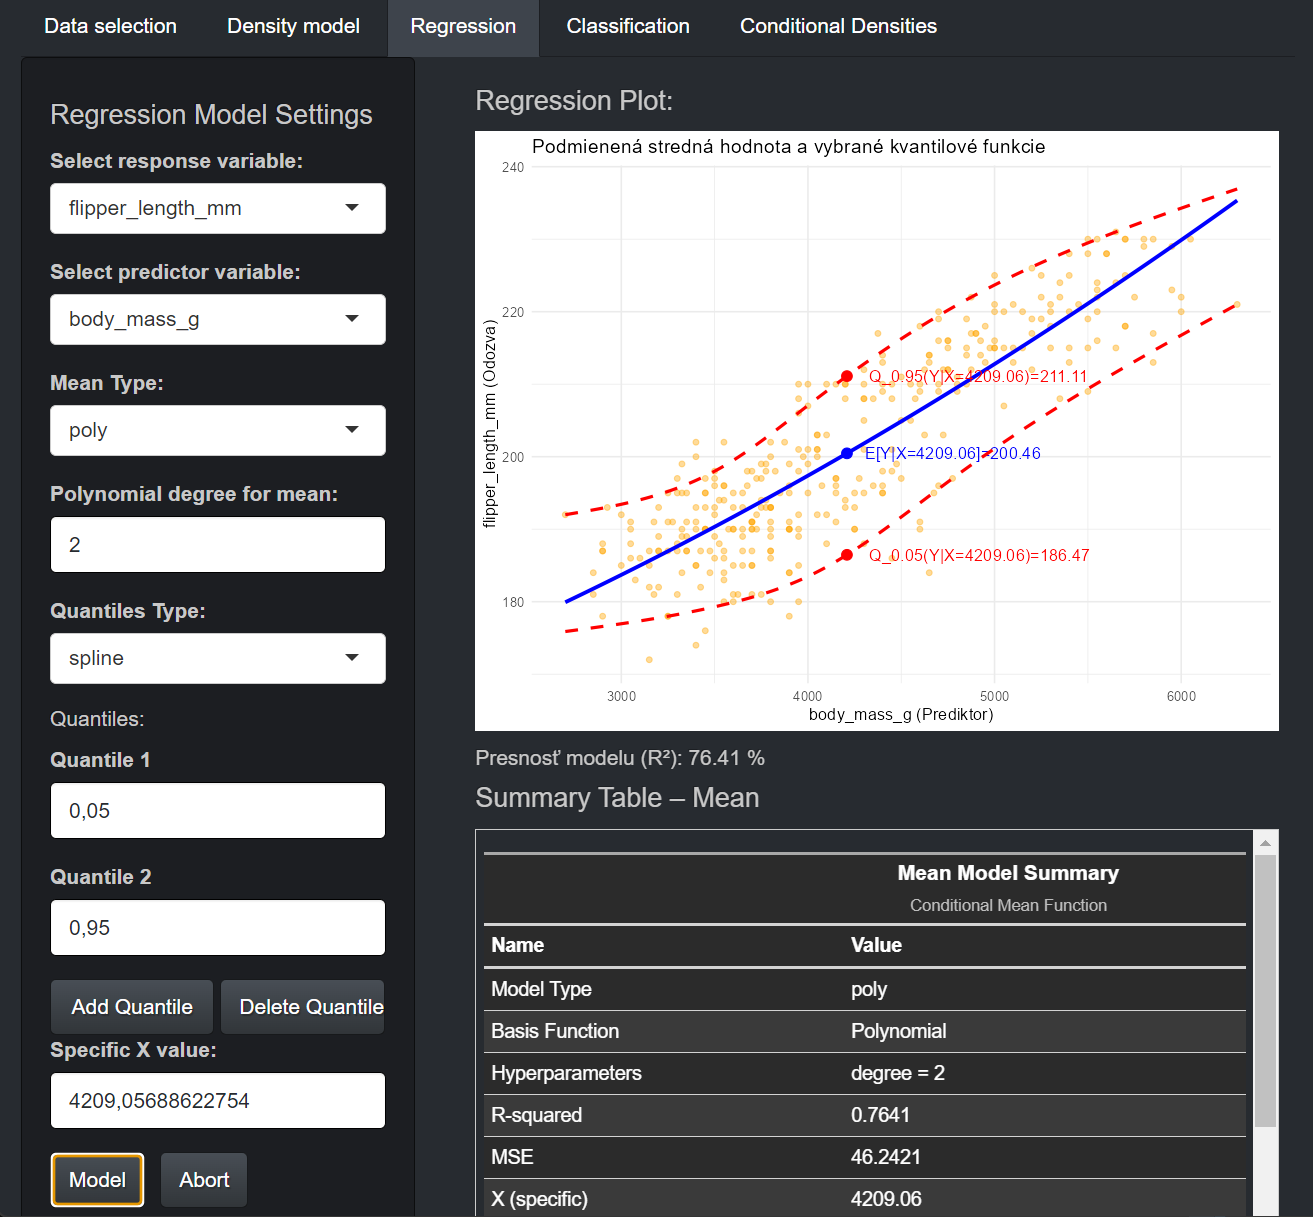
\includegraphics[width=0.75\linewidth]{preview_regression_part1.png}
    \caption{Ukážka výstupu regresného modelu - 1.časť}
    \subcaption{Odozva $Y$: \texttt{Dĺžka krídel}, Prediktor $X$: \texttt{Hmotnosť} + Kvantilové krivky $Q_{Y \mid X}(0.05)$ a $Q_{Y \mid X}(0.95)$ modelované metódou \texttt{"spline"} + stredná hodnota $\mathbb{E}[Y \mid X]$ modelovaná ako polynomiálna funkcia 2. stupňa}
    \label{fig:preview_regression_part1}
\end{figure}

\begin{figure}[H]
    \centering
    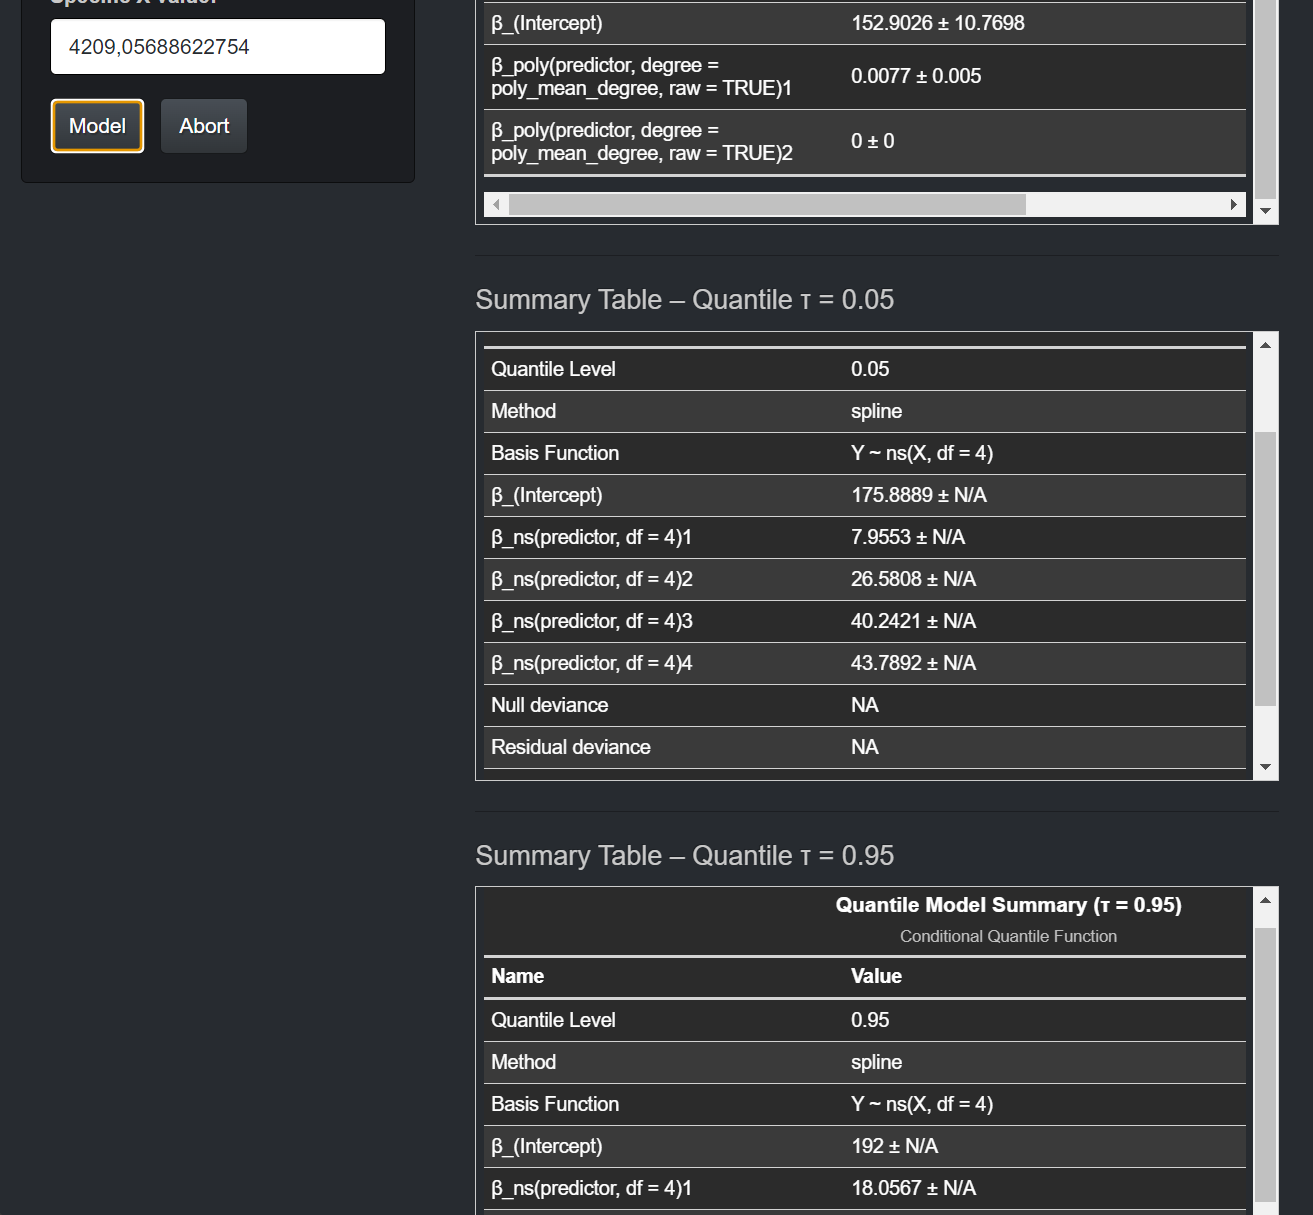
\includegraphics[width=0.75\linewidth]{preview_regression_part2.png}
    \caption{Ukážka výstupu regresného modelu - 2.časť}
    \label{fig:preview_regression_part2}
\end{figure}

\subsection{Klasifikačný model}

\begin{figure}[H]
    \centering
    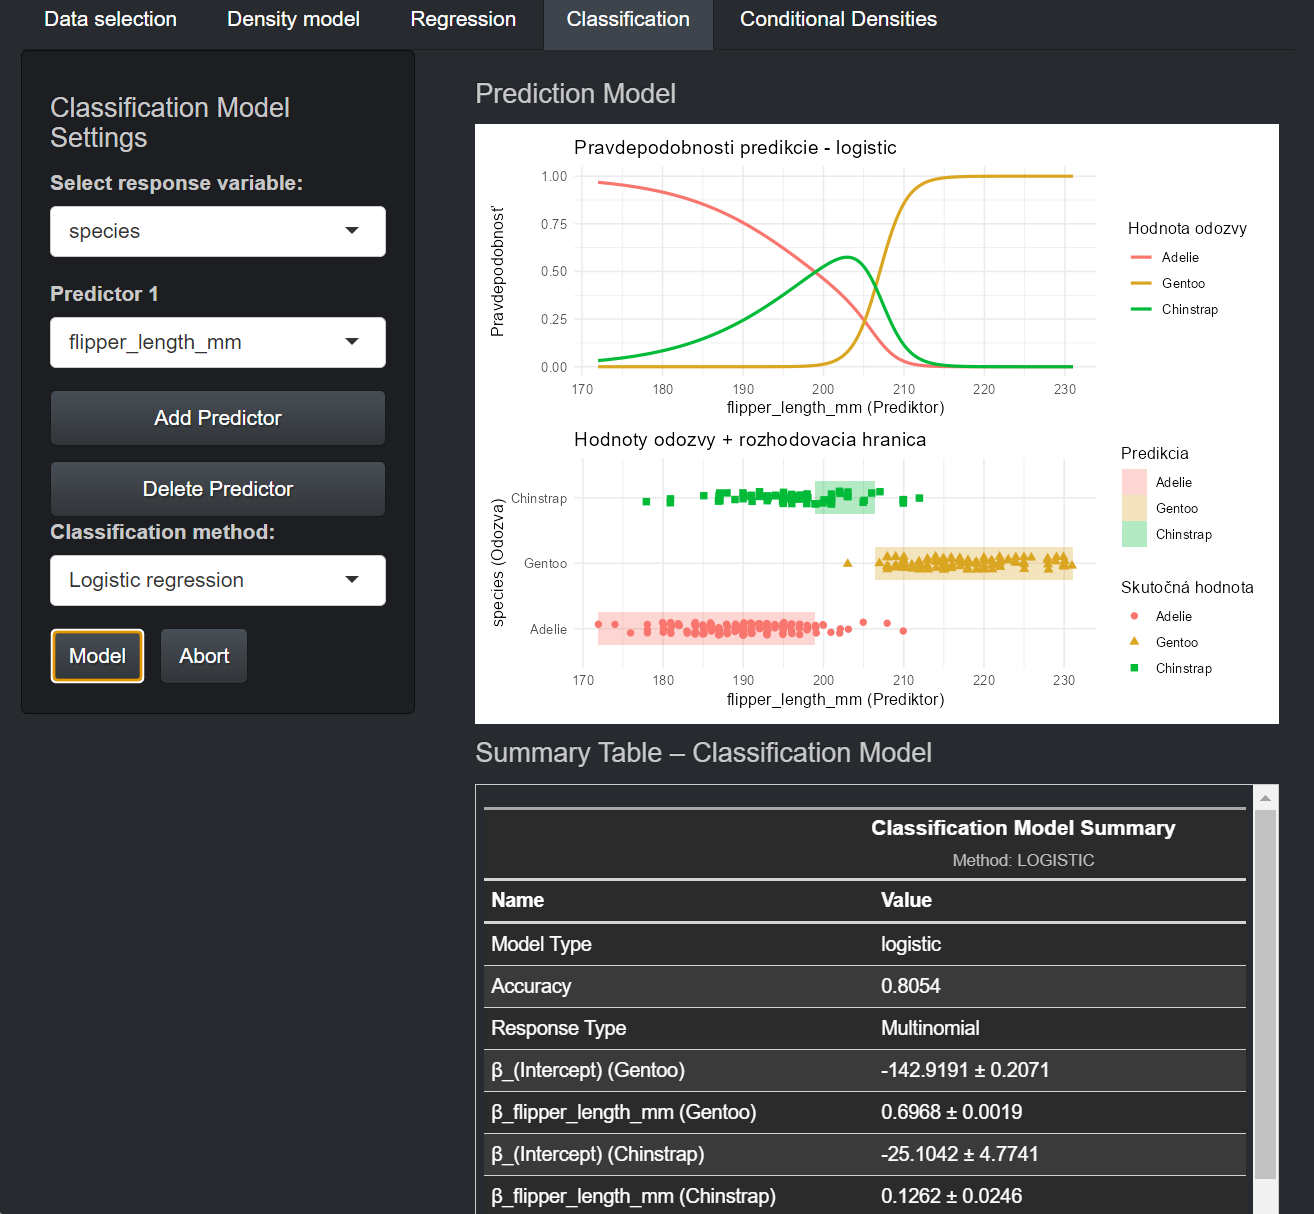
\includegraphics[width=0.7\linewidth]{preview_classification.png}
    \caption{Ukážka výstupu klasifikačného modelu}
    \subcaption{Odozva $Y$: \texttt{Druh}, Prediktor $X$: \texttt{Dĺžka krídel} + Metóda: Logistická regresia(\texttt{"logistic"})}
    \label{fig:preview_classification}
\end{figure}

\subsection{Združené rozdelenie}

\begin{figure}[H]
    \centering
    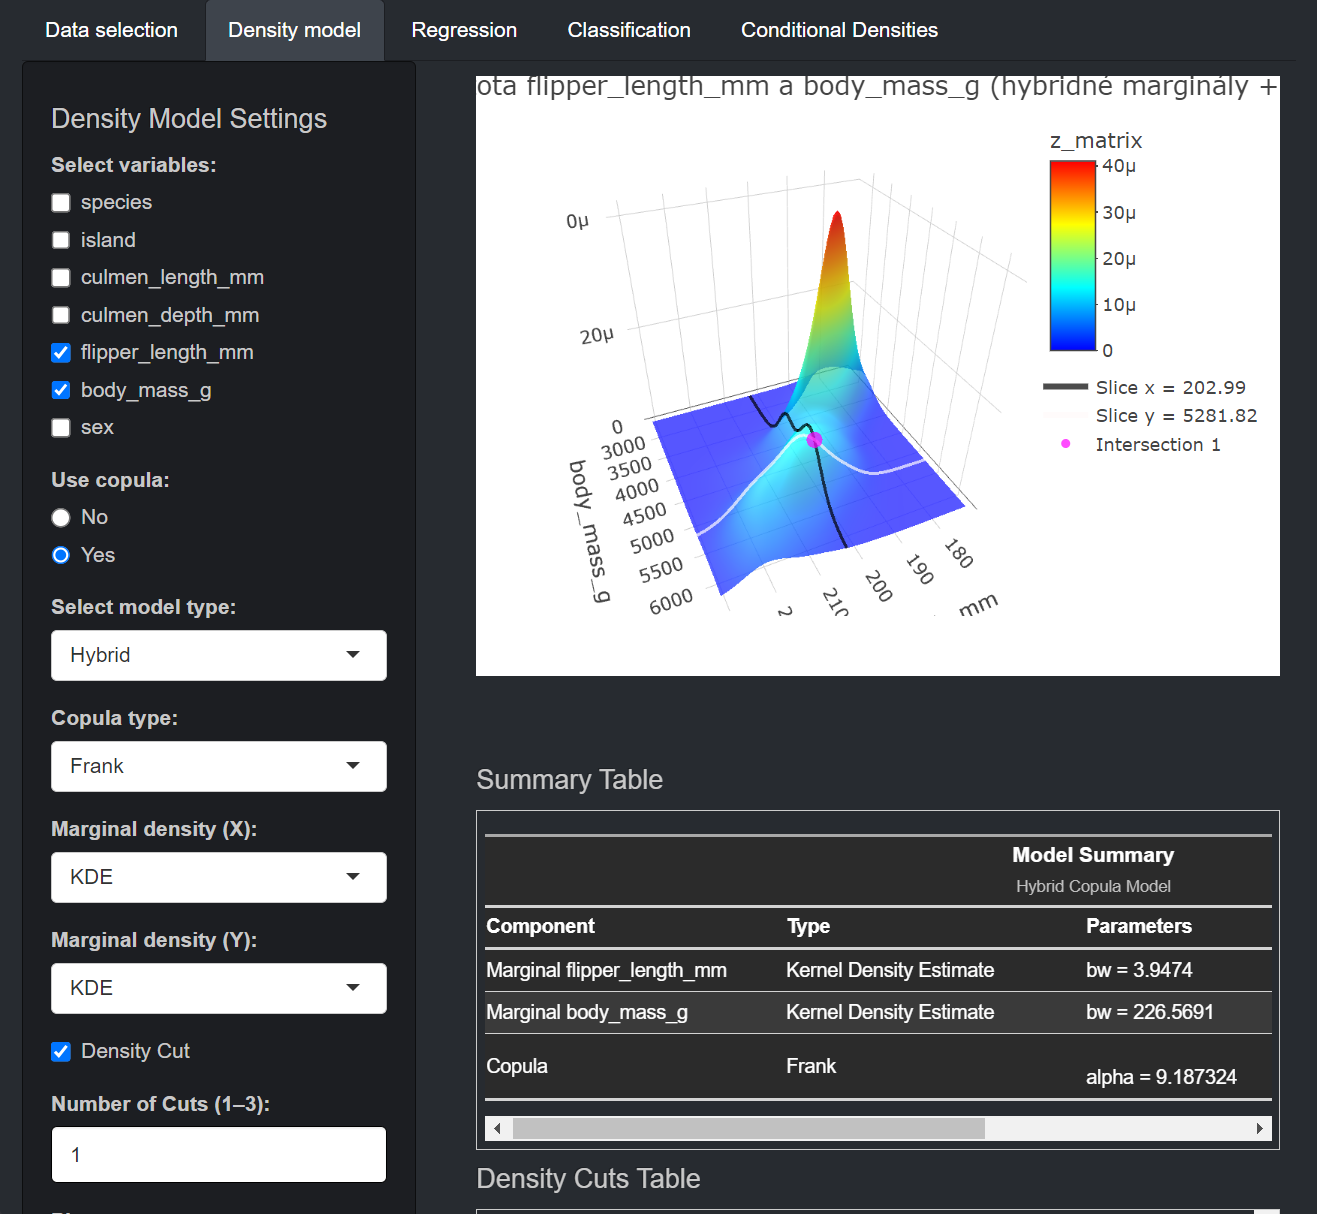
\includegraphics[width=0.65\linewidth]{preview_joint_dist_cont.png}
    \caption{Ukážka 3D výstupu združenej hustoty pravdepodobnosti - spojitý vektor}
    \subcaption{Premenné: \texttt{Hmotnosť} a \texttt{Dĺžka krídel} - modelované cez rozklad na marginálie(odhad obidvoch cez KDE) a kopulu(Frank) + rezy touto hustotou vo vybranom bode}
    \label{fig:preview_joint_dist_cont}
\end{figure}

\begin{figure}[H]
    \centering
    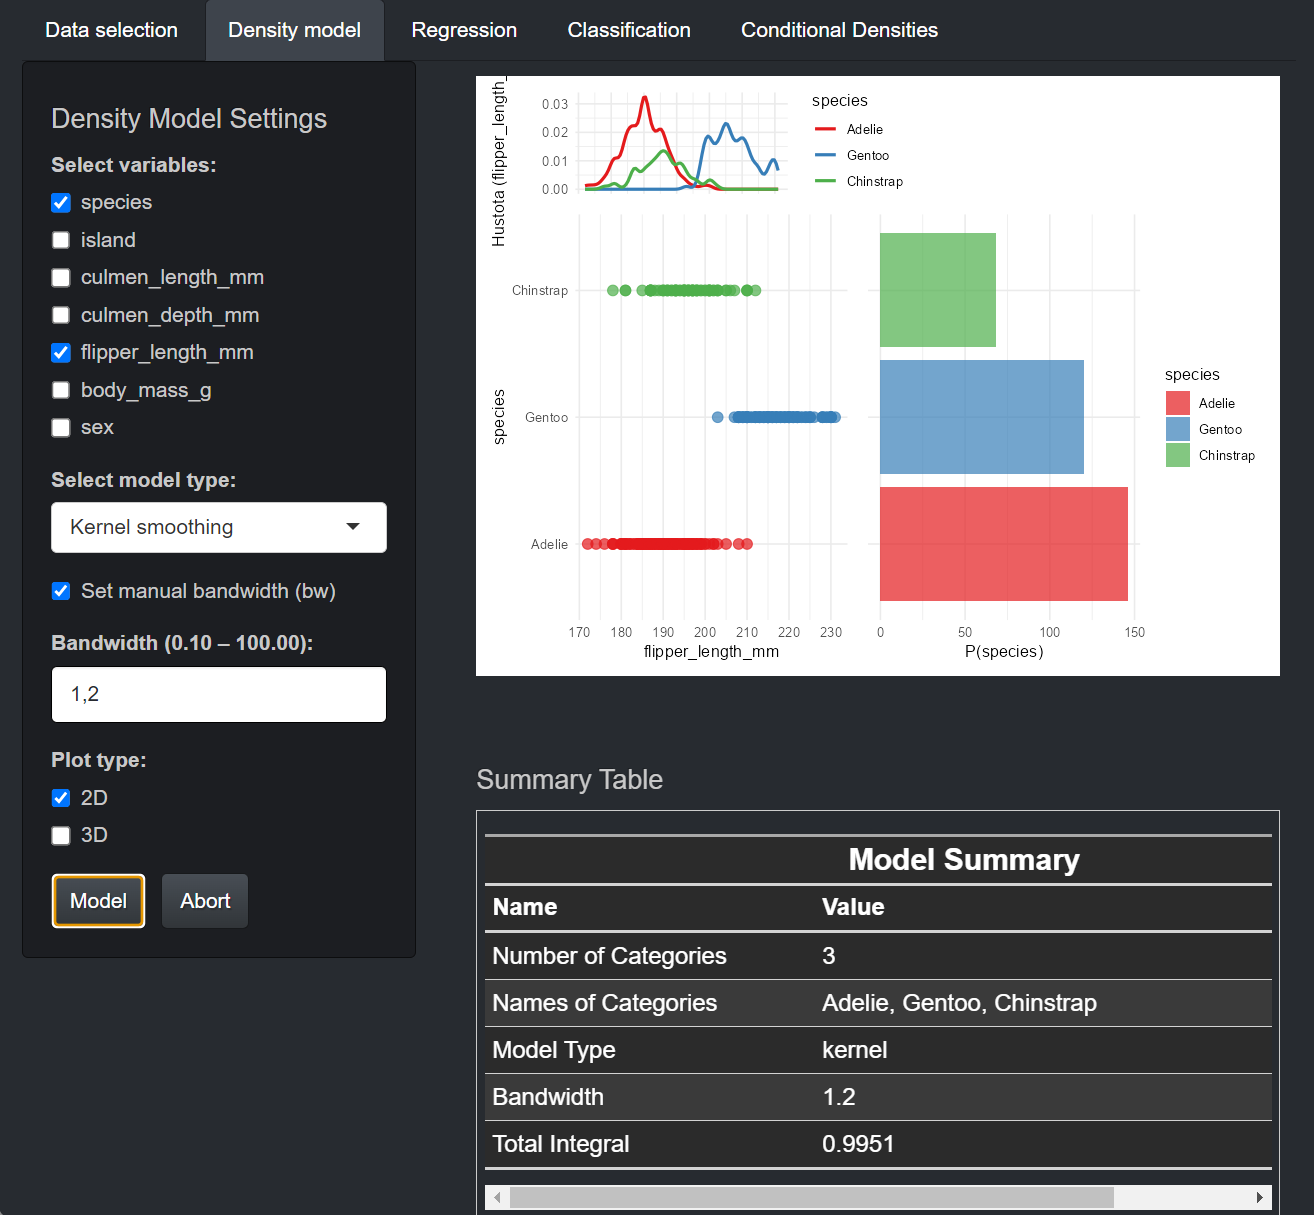
\includegraphics[width=0.65\linewidth]{preview_joint_dist_mix.png}
    \caption{Ukážka 2D výstupu združenej hustoty pravdepodobnosti - zmiešaný vektor}
    \subcaption{Premenné: \texttt{Druh} a \texttt{Dĺžka krídel} - hustoty modelované pomocou jadrového vyhladzovania}
    \label{fig:preview_joint_dist_mix}
\end{figure}

\subsection{Aplikácie združeného rozdelenia}

\begin{figure}[H]
    \centering
    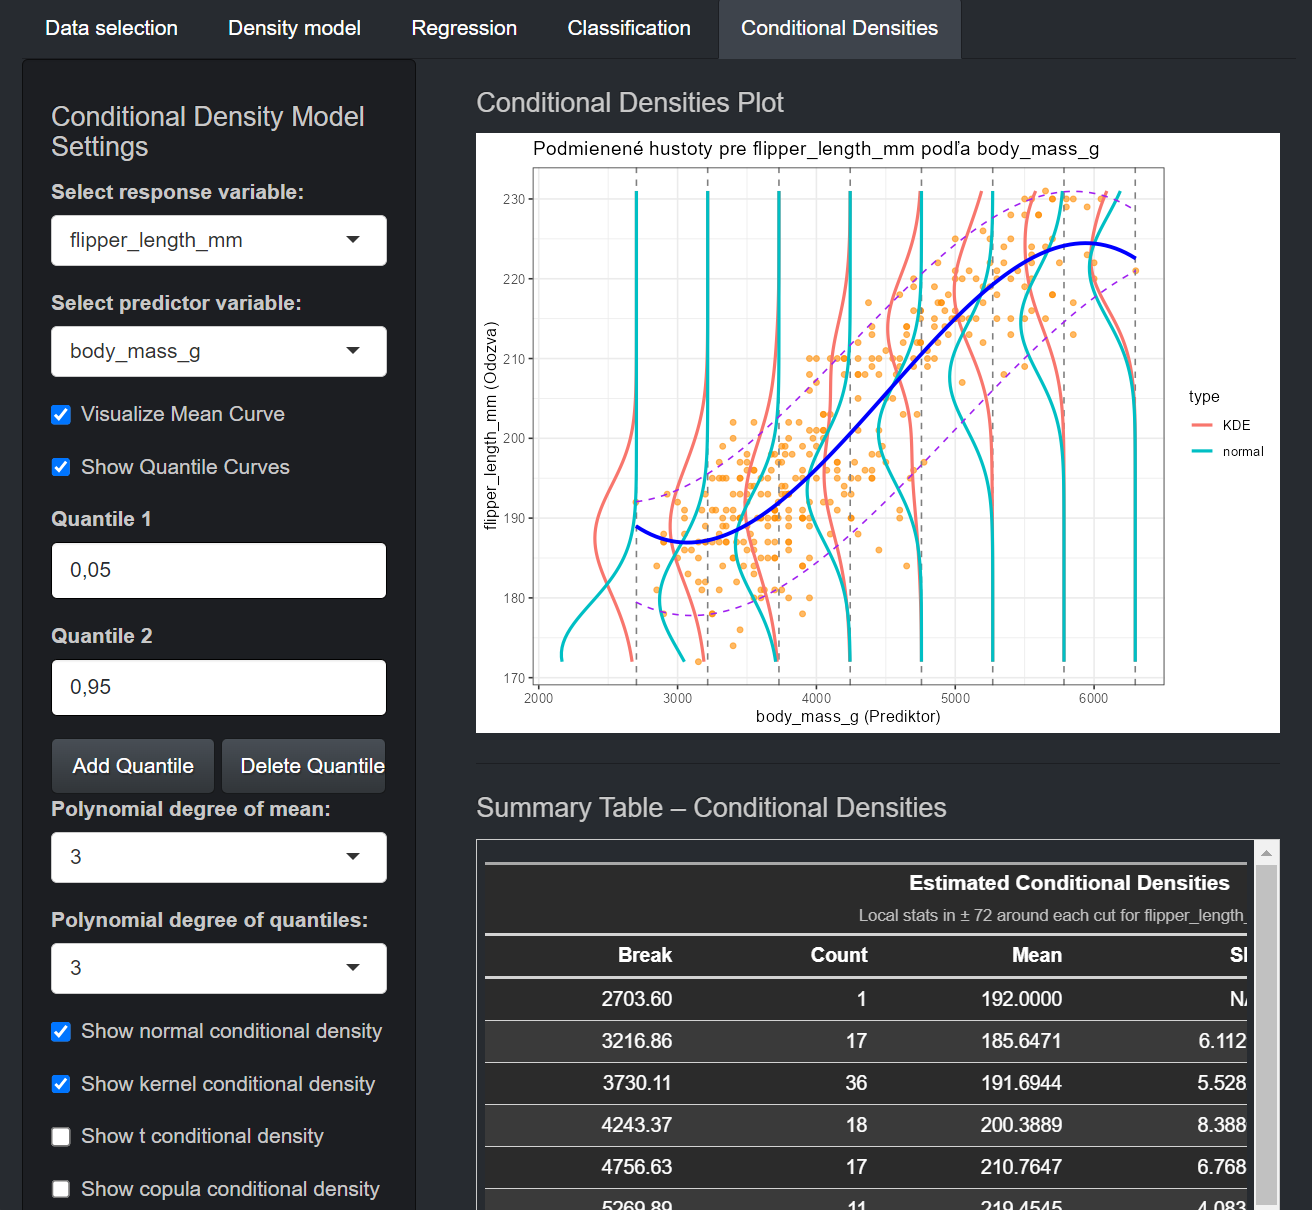
\includegraphics[width=0.65\linewidth]{preview_cond_dens.png}
    \caption{Ukážka výstupu podmieňovania združeného rozdelenia - spojitý vektor}
    \subcaption{Premenné: \texttt{Hmotnosť} a \texttt{Dĺžka krídel} - hustoty modelované pomocou jadrového vyhladzovania (červené) a ako normálne rozdelenie (modré) + kubická podmienená stredná hodnota (tmavomodrá krivka) a kubické kvantilové funkcie (fialové čiarkované krivky)}
    \label{fig:preview_cond_dens}
\end{figure}

\begin{figure}[H]
    \centering
    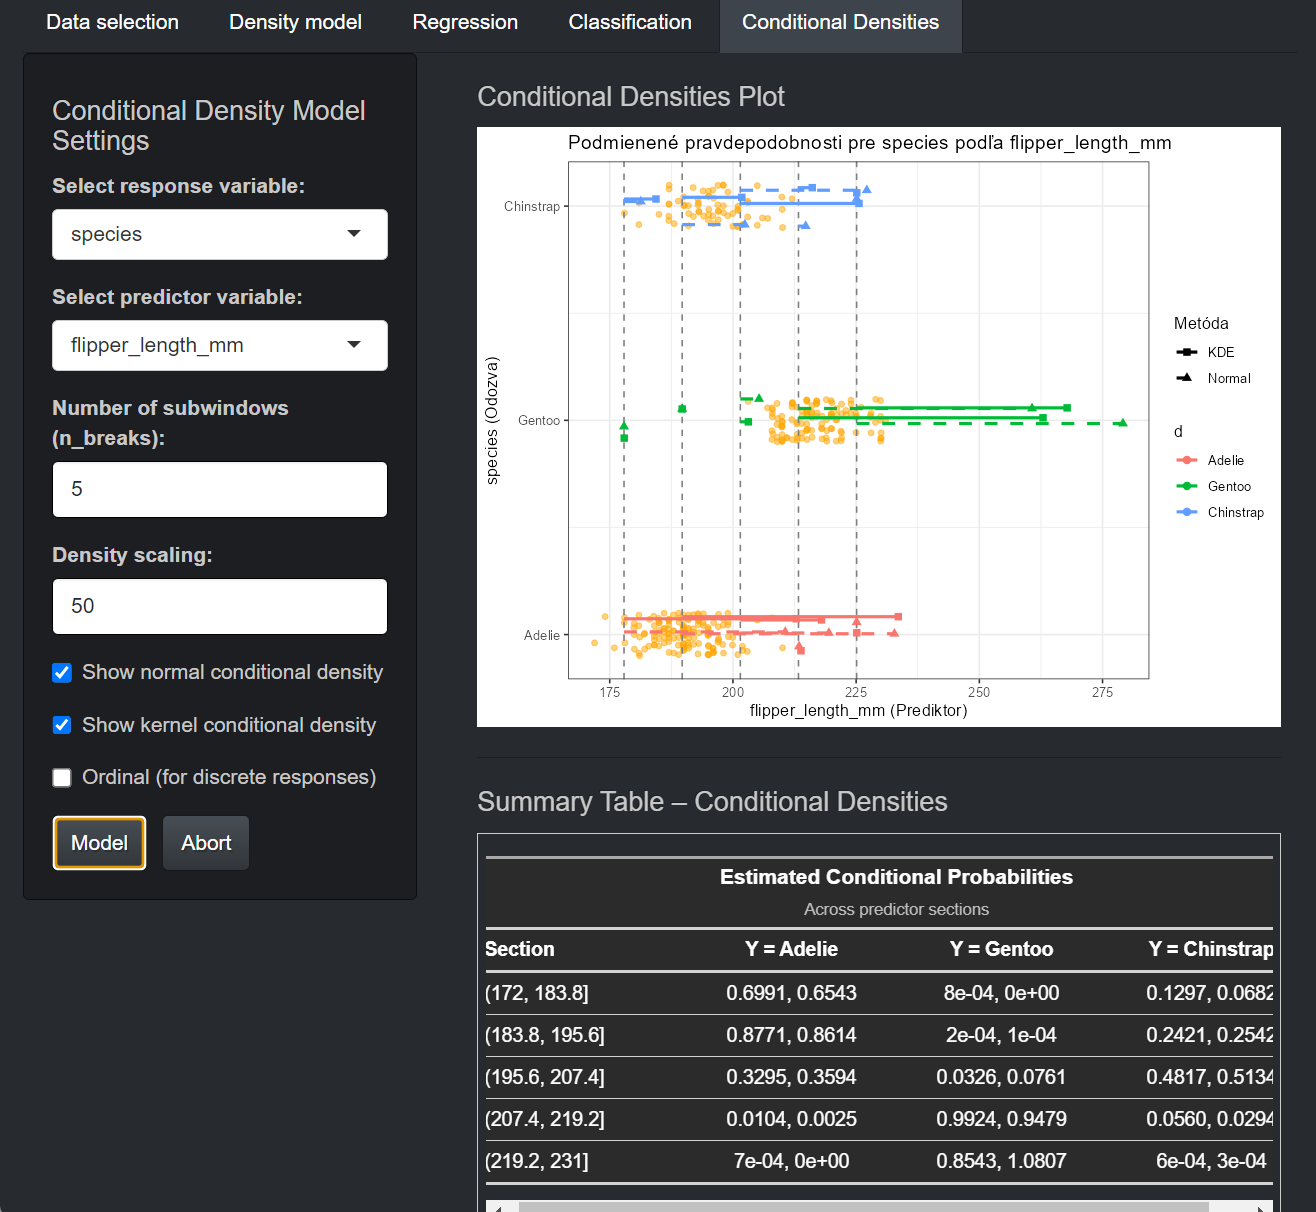
\includegraphics[width=0.65\linewidth]{preview_cond_prob.png}
    \caption{Ukážka výstupu podmieňovania združeného rozdelenia - zmiešaný vektor}
    \subcaption{Premenné: \texttt{Druh} a \texttt{Dĺžka krídel} - pravdepodobnosti modelované z podmienených hustôt pomocou KDE (neprerušované so štvorcom) a ako normálne rozdelenie (prerušované s trojuholníkom)}
    \label{fig:preview_cond_prob}
\end{figure}